\documentclass{article}
\usepackage{listings}
%
\usepackage{makeidx}  % allows for indexgeneration
\usepackage{float}
%
\usepackage[utf8x]{inputenc}
\usepackage[russian]{babel}
\usepackage{indentfirst}
\usepackage{graphicx} % Allows including images
\usepackage{booktabs} % Allows the use of \toprule, \midrule and \bottomrule in tables
\usepackage{caption}
\usepackage{amsmath}
\usepackage{amsfonts}
\usepackage{textcomp}
\usepackage{xcolor}
\usepackage{multirow}
\usepackage{amssymb}


\definecolor{cloudwhite}{HTML}{E9E9E2}
\lstloadlanguages{C,C++,csh,Java}

\definecolor{red}{rgb}{0.6,0,0}
\definecolor{blue}{rgb}{0,0,0.6}
\definecolor{green}{rgb}{0,0.8,0}
\definecolor{cyan}{rgb}{0.0,0.6,0.6}

\lstset{
language=csh,
basicstyle=\footnotesize\ttfamily,
numbers=left,
numberstyle=\tiny,
numbersep=5pt,
tabsize=2,
extendedchars=true,
breaklines=true,
frame=b,
stringstyle=\color{blue}\ttfamily,
showspaces=false,
showtabs=false,
xleftmargin=17pt,
framexleftmargin=17pt,
framexrightmargin=5pt,
framexbottommargin=4pt,
commentstyle=\color{green},
morecomment=[l]{//}, %use comment-line-style!
morecomment=[s]{/*}{*/}, %for multiline comments
showstringspaces=false,
morekeywords={ def, for, from, up, to, by, solve, paa, translate, rotate, around, ->},
keywordstyle=\color{cyan},
identifierstyle=\color{red},
backgroundcolor=\color{cloudwhite},
}

\usepackage{caption}
\DeclareCaptionFont{white}{\color{white}}
\DeclareCaptionFormat{listing}{\colorbox{blue}{\parbox{\textwidth}{\hspace{15pt}#1#2#3}}}
\captionsetup[lstlisting]{format=listing,labelfont=white,textfont=white, singlelinecheck=false, margin=0pt, font={bf,footnotesize}}

\begin{document}

\section{Графический интерфейс}

\begin{figure}[H]
  \centering
  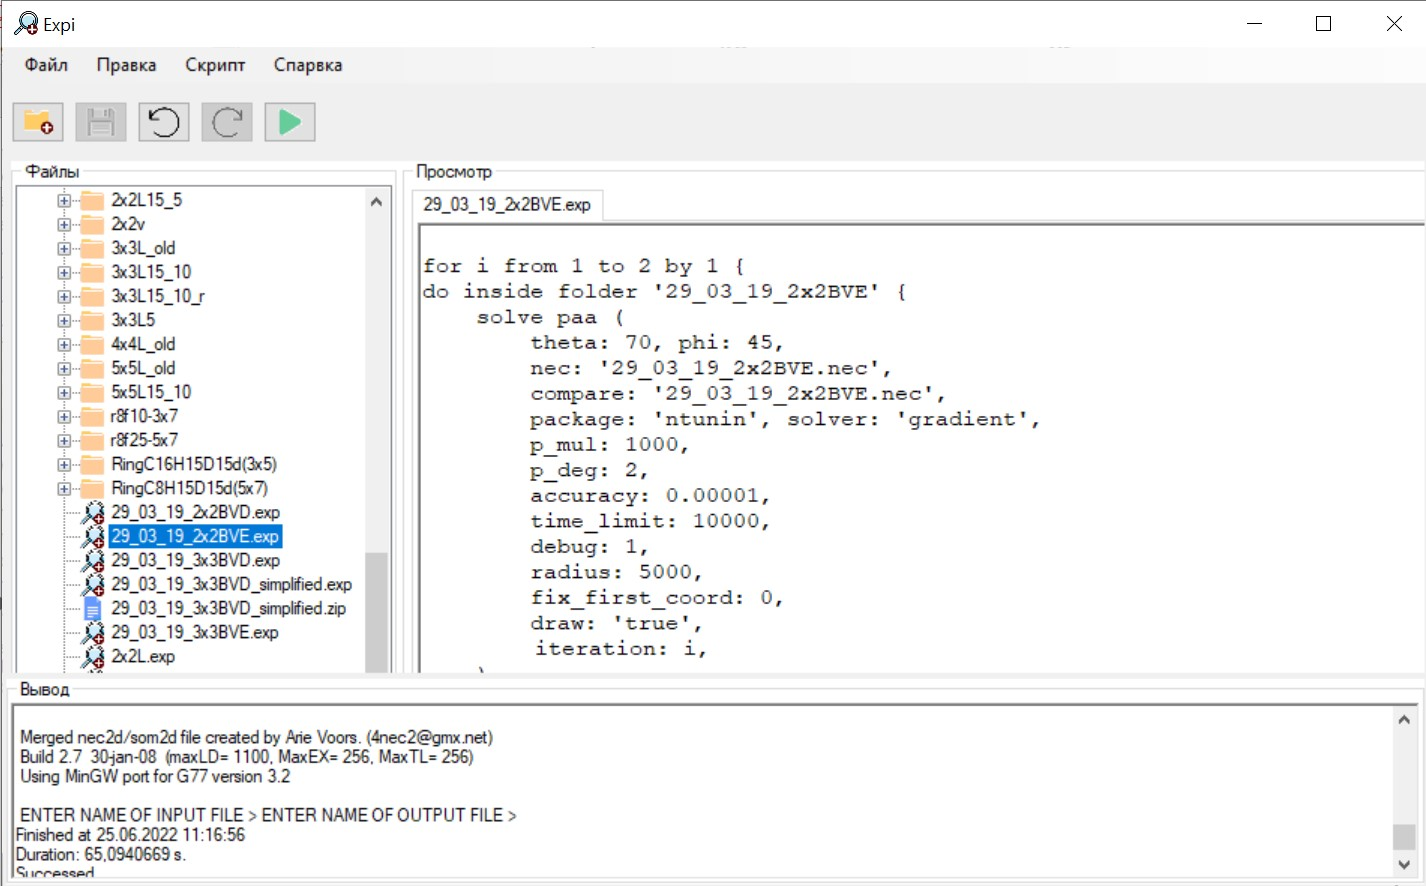
\includegraphics[width=\linewidth]{expi_script.jpeg}
  \caption{Редактор исполняемых файлов}
\end{figure}

\begin{figure}[H]
  \centering
  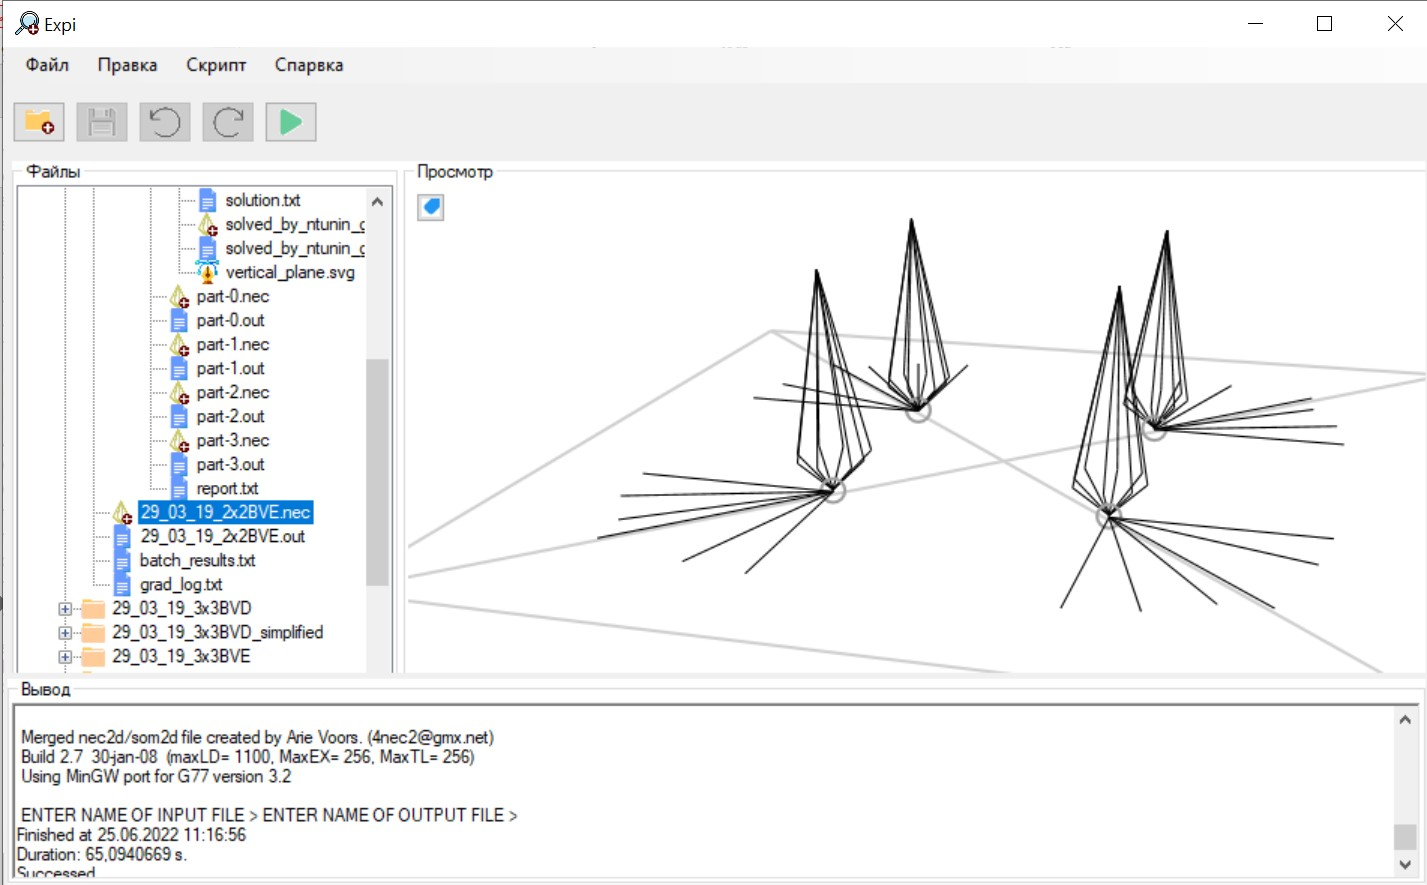
\includegraphics[width=\linewidth]{expi_paa.jpeg}
  \caption{Предпросмотр геометрии}
\end{figure}

\begin{figure}[H]
  \centering
  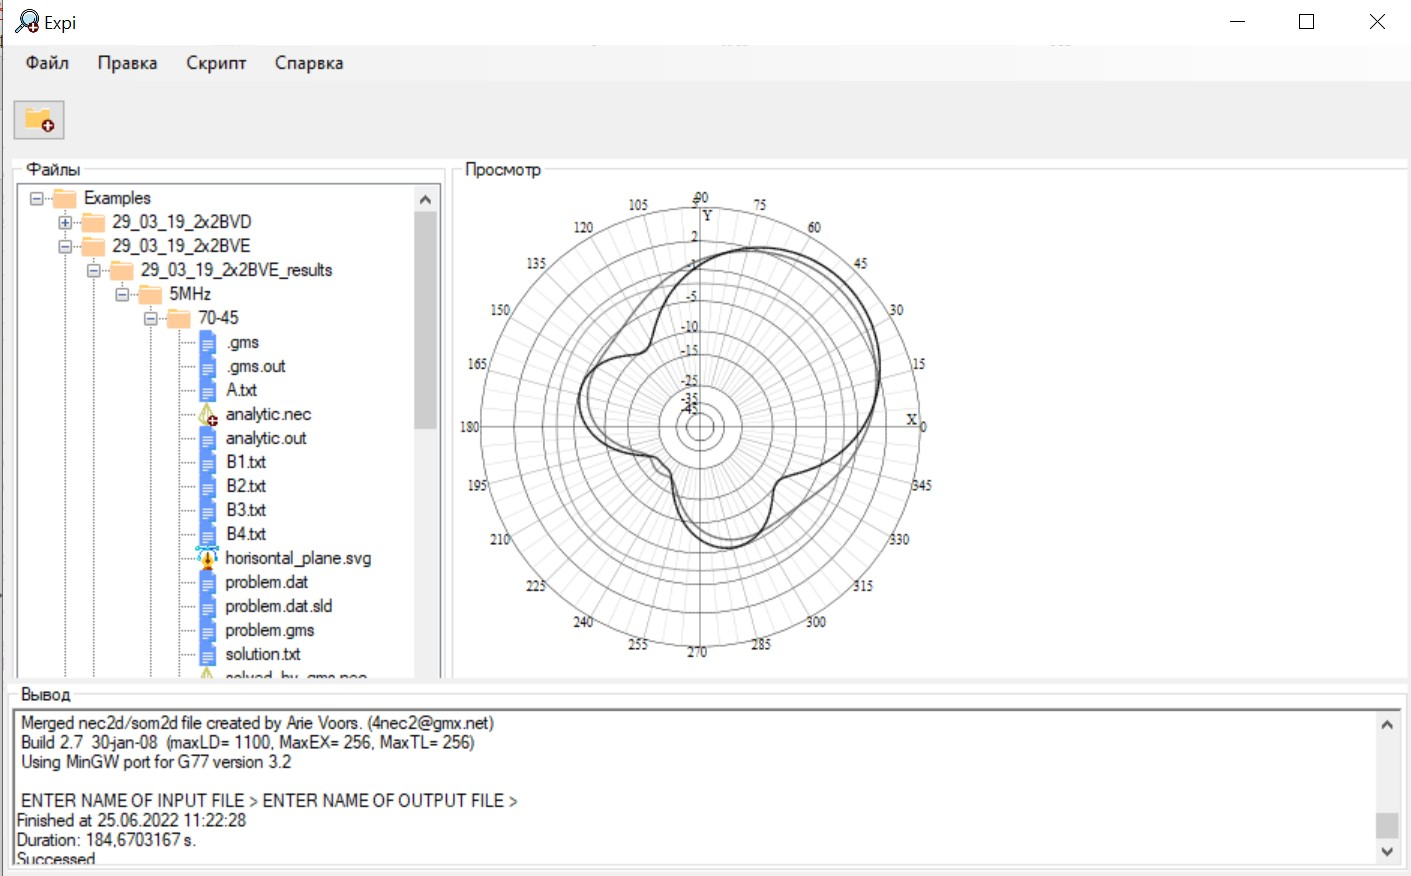
\includegraphics[width=\linewidth]{expi_results.jpeg}
  \caption{Предпросмотр результатов}
\end{figure}

\section{Языковые конструкции}

\begin{lstlisting}[caption={Переменные}, label={experiment}]
def x = 1
def point = (0, 0, 1)
\end{lstlisting}

\begin{lstlisting}[caption={Сегментированный провод}, label={experiment}]
(0, 0, 0) -> (1, 0, 1) -> (0, 0, 5)
(0, 0, 0) -> (1, 0, 1) ~1v~ (0, 0, 5)
(0, 0, 0) -> (1, 0, 1) ~1+0.5iA~ (0, 0, 5)
\end{lstlisting}

\begin{lstlisting}[caption={Линейные преобразования}, label={experiment}]
translate x to 0.5
translate to (0, 0, 1)
rotate around z by pi/2
\end{lstlisting}

\begin{lstlisting}[caption={Циклы}, label={experiment}]

for angle from 0 to 2 * pi by pi/8 {
   rotate around z by angle
   (0, 0, 0) -> (1, 0, 0)
}

for angle from 0 up to 2 * pi by pi/8 {
   rotate around z by angle
   (0, 0, 0) -> (1, 0, 0)
}

\end{lstlisting}


\begin{lstlisting}[caption={Группы команд}, label={experiment}]
def Emitter {
    for angle from 0 to 2 * pi by pi/8 {
       rotate around z by angle
       (0, 0, 0) -> (1, 0, 0)
    }
}

translate x to -5
Emitter
translate x to 5
Emitter
\end{lstlisting}

\begin{lstlisting}[caption={Оптимизация направленности ФАР}, label={experiment}]
solve paa (
    n: 'bve_2x2.nec',
    theta: 70,
    phi: 45,
    p: 'ntunin',
    s: 'grad',
    c: 'bve.nec',
    p_mul: 1000000,
    p_deg: 4,
    time_limit: 1000,
    accuracy: 0.000001
)
\end{lstlisting}



\begin{lstlisting}[caption={Полный текст примера вычислительного эксперимента}, label={experiment}]

def knees = 8
def height = 15
def kneeWidth = 2.5
def base = 0.5
def rize = 2
def radialsCount = 6
def radialLength = 15
def size = 2
def distance = 20

def Drop {
   def step = 2 * pi / knees
   for angle from 0 to 2 * pi by step {
      rotate around z by angle
      (0, 0, 0) -> (kneeWidth, 0, kneeWidth) -> (0, 0, height)
   }
}

def BVE {
   (0, 0, 0) ~1v~ (0, 0, base)
   def step = pi / 2 / (radialsCount - 1)
   for i from 0 to  radialsCount  by 1 {
       rotate around z by i * step
       (0, 0, 0) -> (radialLength, 0, 0)
   }
   translate z to base
   Drop
}

def PlaceBVE {
   translate to (x, y, 0)
   rotate around z by angle
   BVE
}

def PAA {
   def width = (size - 1) * distance
   def left = -width/2
   def right = width/2
   def top = width/2
   def bottom = -width/2

   PlaceBVE(x: left, y: top, angle: pi / 2)
   PlaceBVE(x: right, y: top, angle: 0)
   PlaceBVE(x: right, y: bottom, angle: -pi / 2)
   PlaceBVE(x: left, y: bottom, angle: pi)
}

def ExportPAA {
    export nec (n: 'bve_${size}x${size}.nec', f: 5, g: 'real') {
        translate z to rize
        PAA
    }
}

def One {
    (0, 0, 0) ~1v~ (0, 0, base)
    def oneRadialsCount = (radialsCount - 1) * 4
    def step = 2 * pi / (oneRadialsCount - 1)
    for i from 0 to  oneRadialsCount by 1 {
        rotate around z by i * step
        (0, 0, 0) -> (radialLength, 0, 0)
    }
    translate z to base
    Drop
}

def ExportOne {
    export nec (n: 'bve.nec', f: 5, g: 'real') {
        translate z to rize
        One
    }
}

do inside folder '05.04.22' {
    ExportOne
    ExportPAA

    solve paa (
        n: 'bve_${size}x${size}.nec',
        theta: 70,
        phi: 45,
        p: 'ntunin',
        s: 'grad',
        c: 'bve.nec',
        p_mul: 1000000,
        p_deg: 4,
        time_limit: 1000,
        accuracy: 0.000001
    )
    solve paa (
        n: 'old_bve_${size}x${size}.nec',
        theta: 70,
        phi: 45,
        p: 'ntunin',
        s: 'grad',
        c: 'bve.nec',
        p_mul: 1000000,
        p_deg: 4,
        time_limit: 1000,
        accuracy: 0.000001
    )
}

\end{lstlisting}

\end{document} 